\chapter{Các công trình và công cụ liên quan}

% Tick/cross/warning macros cho các bảng so sánh
\newcommand{\yesmark}{\ding{51}}
\newcommand{\nomark}{\ding{55}}
\newcommand{\partialmark}{\ding{109}}

Chương này gồm hai phần. Phần thứ nhất khảo sát các \textit{công trình nghiên cứu liên quan} theo bốn hướng tiếp cận gần với đề tài: CSPM truyền thống và CNAPP thương mại, các framework điều phối agentic workflow (Compound AI System), các nghiên cứu LLM cho an ninh mạng, và các khung đánh giá Security Maturity tự động. Phần thứ hai trình bày các \textit{công cụ tích hợp} (Prowler, LangChain, LangGraph, Ollama, Boto3, ChromaDB) được sử dụng làm hạ tầng cho hệ thống đề xuất, cùng vai trò cụ thể của từng công cụ trong kiến trúc tổng thể. Chương kết thúc bằng phần định vị đề tài trong không gian thiết kế hiện có.

\section{Các công trình nghiên cứu liên quan}
\label{sec:related-research}

Bài toán tự động hóa đánh giá và khắc phục bảo mật trên đám mây có thể được tiếp cận theo bốn hướng nghiên cứu chính: (i) các nền tảng CSPM truyền thống và CNAPP thương mại tập trung vào phát hiện cấu hình sai và ưu tiên hoá rủi ro; (ii) các framework điều phối agentic workflow dạng Compound AI System hướng tới khả năng lập kế hoạch, suy luận và gọi công cụ qua LLM; (iii) các nghiên cứu trực tiếp ứng dụng LLM cho kiểm toán bảo mật và tuân thủ; và (iv) các khung đánh giá Security Maturity định lượng mức trưởng thành an ninh. Mỗi hướng có những đóng góp và hạn chế riêng; phần này phân tích các đại diện tiêu biểu, từ đó làm nổi bật khoảng trống mà đề tài hướng tới lấp đầy.

\subsection{Cloud Security Posture Management (CSPM) truyền thống}
\label{subsec:rw-cspm}

CSPM \cite{gartner_cspm} là một lớp giải pháp được Gartner định nghĩa nhằm đánh giá và giám sát liên tục cấu hình bảo mật của các tài nguyên đám mây. Một trong những công trình học thuật tiêu biểu về CSPM là \textbf{CSBAuditor} của Torkura và cộng sự \cite{torkura2019csbauditor} — hệ thống chủ động phân tích rủi ro cho các Cloud Storage Broker, sử dụng cơ chế kiểm tra liên tục dựa trên rule-set tĩnh để phát hiện cấu hình lệch chuẩn. CSBAuditor nhấn mạnh khía cạnh phát hiện và cảnh báo, không tích hợp khâu khắc phục tự động.

Trong nhóm sản phẩm thương mại và mã nguồn mở, các nền tảng tiêu biểu bao gồm:
\begin{itemize}
    \item \textbf{AWS Security Hub} \cite{aws_securityhub} — dịch vụ CSPM gốc của AWS, tổng hợp các findings từ nhiều dịch vụ con (GuardDuty, Inspector, Macie...) theo các framework tuân thủ (CIS AWS Foundations, PCI-DSS). Hạn chế chính là phụ thuộc vào hạ tầng AWS và không cung cấp khả năng remediation closed-loop ngoài các automation rule do người dùng tự định nghĩa.
    \item \textbf{ScoutSuite} (NCC Group) \cite{scoutsuite} — công cụ kiểm toán đa-cloud thực thi qua API call, xuất báo cáo HTML; thiên về phát hiện, không có pha khắc phục.
    \item \textbf{Cloud Custodian} (Capital One) \cite{cloudcustodian} — rule engine YAML-based cho phép định nghĩa policy bảo mật và đính kèm action remediation cố định. Mạnh ở mức độ tự động hoá hành động, nhưng phụ thuộc vào tập rule do người vận hành biên soạn thủ công và không có cơ chế suy luận ngữ nghĩa.
    \item \textbf{Prowler} \cite{prowler} — công cụ mã nguồn mở agentless với tập checks lớn theo nhiều chuẩn (CIS, NIST, GDPR...). Đề tài này tích hợp Prowler ở vai trò công cụ đánh giá; chi tiết được trình bày ở §\ref{sec:prowler-tool}.
\end{itemize}

\noindent\textbf{Xu hướng hợp nhất CNAPP 2024--2025.} Giai đoạn 2023--2025 chứng kiến sự dịch chuyển của thị trường CSPM thương mại sang mô hình \textit{Cloud-Native Application Protection Platform} (CNAPP) \cite{gartner_cnapp_2024}, hợp nhất ba lớp CSPM, CWPP (Cloud Workload Protection) và CIEM (Cloud Infrastructure Entitlement Management) trong một nền tảng. Các đại diện tiêu biểu gồm \textbf{Wiz}, \textbf{Orca Security}, \textbf{Microsoft Defender for Cloud}, và \textbf{Palo Alto Prisma Cloud}. Điểm chung của các CNAPP này là khả năng phân tích rủi ro dựa trên đồ thị quan hệ tài nguyên (\textit{security graph}) và ưu tiên hoá theo \textit{attack path}. Tuy nhiên, toàn bộ các nền tảng nêu trên đều vận hành dưới dạng dịch vụ SaaS đám mây, đòi hỏi tải dữ liệu cấu hình ra bên thứ ba để phân tích --- không tương thích với ràng buộc \textit{local inference} của đề tài (xem §\ref{subsec:rw-scope}).

\noindent\textit{Hạn chế chung của hướng (i):} các công cụ CSPM truyền thống và CNAPP 2024 đều tập trung vào pha \textit{phát hiện} và \textit{ưu tiên hoá rủi ro}; pha \textit{lập kế hoạch khắc phục} thường được biểu diễn dưới dạng tập rule tĩnh hoặc playbook do người vận hành biên soạn thủ công, thiếu cơ chế suy luận trên ngữ nghĩa của findings và không có vòng \textit{xác minh hậu khắc phục} (post-remediation verification) tích hợp trong cùng một workflow.

\subsection{Compound AI Systems và Agentic Workflow Frameworks}
\label{subsec:rw-agentic}

Bên cạnh CSPM truyền thống, một hướng nghiên cứu mới sử dụng các mô hình ngôn ngữ lớn làm lõi suy luận trong các hệ thống có nhiều bước, có công cụ và có trạng thái. Theo Zaharia và cộng sự \cite{zaharia_compound_2024}, các hệ thống dạng này được định danh là \textit{Compound AI System} --- chất lượng đầu ra phụ thuộc nhiều vào thiết kế quy trình bao quanh mô hình hơn là chỉ vào năng lực mô hình lõi. Cơ sở lý thuyết được trình bày tại §\ref{sec:ai-agent}, gồm mẫu \textbf{ReAct} \cite{yao2023react} đan xen \textit{reasoning} và \textit{acting}, mẫu \textbf{Plan-and-Execute} cho tác vụ dài, và cơ chế \textbf{Tool Use} \cite{schick2023toolformer} cho hành động qua công cụ.

Năm framework đại diện trong giai đoạn 2023--2025:
\begin{itemize}
    \item \textbf{AutoGen} (Microsoft) \cite{microsoft2023autogen} --- framework xây dựng ứng dụng agentic thông qua hội thoại giữa các \textit{agent} được phân vai, với \texttt{UserProxyAgent} làm điểm tích hợp human-in-the-loop. AutoGen hỗ trợ kết nối tới LLM cục bộ qua endpoint OpenAI-compatible. Hạn chế: cơ chế kiểm soát luồng và bền vững hoá trạng thái phụ thuộc vào người triển khai, không có model thực thi xác định ở mức framework.
    \item \textbf{MetaGPT} \cite{hong2024metagpt} --- framework phân vai theo SOP (Standard Operating Procedure) kiểu kỹ sư phần mềm (PM, Architect, Engineer\dots) cho bài toán sinh code. Mô hình hợp tác dựa trên SOP, không phải state machine; không nhằm mục tiêu kiểm toán cấu hình.
    \item \textbf{CrewAI} \cite{crewai_2024} --- framework agentic dựa trên \textit{role}, \textit{goal} và \textit{task} của từng agent, hỗ trợ chế độ tuần tự và song song. Định hướng vào kịch bản agent cộng tác; chưa có cơ chế interrupt và checkpoint ở mức framework để phục vụ workflow audit có HITL.
    \item \textbf{LangGraph} \cite{langgraph2024} --- thư viện điều phối agentic dựa trên đồ thị trạng thái (\textit{StateGraph}), hỗ trợ persistence (SqliteSaver/PostgresSaver), \texttt{interrupt()} cho HITL, conditional cycles, và Send API cho parallel branches. Cung cấp mô hình thực thi xác định và có thể truy vết, phù hợp với các bài toán cần kiểm soát chặt như đánh giá bảo mật.
    \item \textbf{Semantic Kernel} (Microsoft) \cite{semantic_kernel_2024} --- SDK model-agnostic với planner, memory, và plugin abstractions. Phù hợp tích hợp vào hệ sinh thái .NET; mức độ trưởng thành cho workflow agentic phức tạp ngắn hơn LangGraph.
\end{itemize}

\noindent\textit{Vì sao đề tài chọn LangGraph.} Bài toán đánh giá bảo mật theo chu trình PDCA yêu cầu ba tính chất kỹ thuật cốt lõi: (a) \textit{tính xác định} của luồng để kiểm thử và truy vết được; (b) khả năng \textit{interrupt/resume} ở các điểm phê duyệt nhạy cảm (HITL); và (c) cơ chế \textit{persistence} cho trạng thái phiên dài. LangGraph phục vụ trực tiếp ba yêu cầu này thông qua mô hình StateGraph với reducer per-key (xem §\ref{subsec:state-graph}), trong khi AutoGen và CrewAI định hướng vào tương tác đa-vai trò mà không cung cấp đầy đủ ba bảo đảm trên ở mức framework. Bảng so sánh chi tiết các framework được trình bày tại §\ref{subsec:langgraph-tool}.

\subsection{LLM kết hợp với kiểm toán bảo mật và tuân thủ}
\label{subsec:rw-llm-audit}

Hướng nghiên cứu thứ ba tập trung trực tiếp vào việc ứng dụng LLM cho các tác vụ an ninh mạng và kiểm toán. Một số đại diện tiêu biểu trong giai đoạn 2023--2025:
\begin{itemize}
    \item \textbf{PentestGPT} \cite{deng2024pentestgpt} — tác tử LLM cho kiểm thử xâm nhập (penetration testing). Tác tử phân tích mục tiêu, chia nhỏ thành các bước con và tự động sinh lệnh; đánh giá được công bố tại USENIX Security 2024 cho thấy khả năng giải các bài tập CTF thực tế.
    \item \textbf{Khảo sát của Ferrag và cộng sự về Generative AI cho an ninh mạng} \cite{ferrag2024genai_cybersec} — tổng hợp các ứng dụng LLM trong phát hiện mã độc, phân tích lỗ hổng, kiểm thử và tuân thủ; chỉ ra các thách thức về độ tin cậy, prompt injection và tính có thể truy vết.
    \item \textbf{Tài liệu AWS Security Maturity Model} \cite{aws_smm} — không phải công trình LLM nhưng cung cấp khung trưởng thành cho an ninh AWS theo bốn giai đoạn (\textit{Quick Wins}, \textit{Foundational}, \textit{Efficient}, \textit{Optimized}); là tài liệu nguồn được lập chỉ mục vào kho RAG của đồ án để phục vụ giai đoạn lập kế hoạch và đánh giá rủi ro.
\end{itemize}

\noindent\textbf{Đánh giá định hướng phương pháp luận.} Phần lớn các công trình kể trên được đánh giá bằng các metric đặc thù của riêng mỗi tác vụ (task success rate trên CTF cho PentestGPT; F1 phân loại malware cho khảo sát của Ferrag) và \textbf{không} sử dụng các metric đặc thù cho phòng ngự cấu hình như \textit{compliance coverage}, \textit{false-remediation rate}, hoặc \textit{security score delta} (xem §\ref{subsec:eval-security}). Vì vậy, kết quả từ các công trình này không thể chuyển trực tiếp làm baseline cho bài toán CSPM closed-loop --- một khoảng trống về \textit{phương pháp đánh giá} sẽ được đề tài đề xuất xử lý ở Chương~6.

\noindent\textbf{Vị trí của các paradigm RAG mới.} Các paradigm RAG 2024 (\textit{Self-RAG}, \textit{GraphRAG}, \textit{Adaptive-RAG}; xem §\ref{subsec:rag-2024}) chưa được áp dụng phổ biến cho miền tri thức bảo mật do hai rào cản: (i) Self-RAG đòi hỏi fine-tune mô hình với reflection tokens, không khả thi với SLM cục bộ ở phạm vi đề tài; (ii) GraphRAG yêu cầu xây trước knowledge graph từ corpus, chi phí offline cao và cần định nghĩa entity/relation schema cho miền CSPM. Do đó đề tài chọn hướng \textit{Hybrid retrieval} (BM25 + Dense + RRF) kết hợp \textit{metadata filtering} --- thiết kế này đặt mục tiêu trade-off khác: latency thấp, không yêu cầu fine-tune, và tận dụng metadata cấu trúc của corpus CSPM.

\noindent\textit{Hạn chế chung của hướng (iii):} hầu hết các công trình LLM cho an ninh mạng tập trung vào kiểm thử tấn công (offensive) hoặc phát hiện mã độc; số lượng nghiên cứu áp dụng LLM cho \textit{phòng ngự cấu hình} (CSPM) theo chu trình closed-loop còn hạn chế. Đặc biệt, đa số kiến trúc dựa trên LLM thương mại (GPT-4, Claude\dots) qua API đám mây, không tương thích với yêu cầu \textit{local inference} để bảo vệ tính riêng tư của dữ liệu cấu hình hạ tầng (giả định được phát biểu rõ tại §\ref{subsec:rw-scope}).

\subsection{Đánh giá Security Maturity tự động}
\label{subsec:rw-maturity}

Đề tài có khái niệm trung tâm là \textit{Security Maturity} --- xuất hiện trong tiêu đề luận văn. Cần phân biệt rõ giữa hai loại đánh giá thường bị lẫn lộn: (i) \textit{compliance assessment} --- so sánh cấu hình hiện tại với tập kiểm soát chuẩn theo tỉ lệ \textit{pass/fail}, đầu ra là số phần trăm phủ; (ii) \textit{maturity assessment} --- định vị tổ chức theo \textit{bậc} năng lực (thường 4--5 mức từ \textit{Initial} đến \textit{Optimizing}), đầu ra là một mức trưởng thành theo từng lĩnh vực kiểm soát \cite{sei_cmm_1993}. Phần lớn công cụ CSPM khảo sát ở §\ref{subsec:rw-cspm} thuộc loại (i); các work liên quan đến (ii) tạo thành một hướng riêng và được phân tích dưới đây.

\subsubsection*{Maturity models cho an toàn phần mềm}

Hai khung tham chiếu phổ biến nhất bắt nguồn từ engineering security:
\begin{itemize}
  \item \textbf{BSIMM} (Building Security In Maturity Model) \cite{bsimm_v14} --- chương trình khảo sát thường niên của Synopsys với 12 \textit{practices} chia thành bốn domain (Governance, Intelligence, SSDL Touchpoints, Deployment). Mỗi practice có 3 mức trưởng thành. Khảo sát BSIMM 14 (2024) công bố dữ liệu từ ~130 tổ chức tham gia.
  \item \textbf{OWASP SAMM v2} \cite{owasp_samm_v2} --- mô hình mã nguồn mở với 5 business function (Governance, Design, Implementation, Verification, Operations), mỗi business function có 3 security practice và 3 maturity level. So với BSIMM, SAMM nhẹ hơn và phù hợp tự đánh giá.
  \item \textbf{OWASP DSOMM} \cite{owasp_dsomm} --- DevSecOps Maturity Model, mở rộng SAMM cho ngữ cảnh CI/CD và infrastructure-as-code. Có ý nghĩa đặc biệt với phần \textit{infrastructure security} (gần với CSPM).
\end{itemize}

\subsubsection*{Maturity models cho hạ tầng và critical infrastructure}

\begin{itemize}
  \item \textbf{NIST Cybersecurity Framework Implementation Tiers} \cite{nist_csf_2024} --- 4 tier (Partial, Risk Informed, Repeatable, Adaptive) đặt ngang với 6 chức năng của CSF v2.0. Đây là khung tham chiếu phổ biến nhất ở mức quản trị.
  \item \textbf{DOE C2M2 v2.1} \cite{c2m2_v2_1} --- mô hình của Bộ Năng lượng Hoa Kỳ cho hạ tầng năng lượng/critical infrastructure, gồm 10 domain với 4 mức Maturity Indicator Level (MIL0--MIL3).
  \item Khảo sát hệ thống của Rea-Guaman và cộng sự \cite{rea2020cyber_maturity_systematic} so sánh đa khung trưởng thành an ninh mạng và chỉ ra sự thiếu vắng \textit{định lượng tự động} là khoảng trống chung.
\end{itemize}

\subsubsection*{Maturity models cho đám mây}

\begin{itemize}
  \item \textbf{AWS Security Maturity Model} \cite{aws_smm} --- bốn giai đoạn (Quick Wins, Foundational, Efficient, Optimized) gắn trực tiếp với dịch vụ AWS; là khung mà đề tài chọn làm kim chỉ nam cho mô hình hoá Maturity Score, trước mắt được áp dụng và kiểm chứng end-to-end trên dịch vụ S3.
  \item \textbf{AWS Well-Architected Framework --- Security Pillar} \cite{aws_well_architected_security} --- whitepaper ưu tiên best practices nhưng không có thang trưởng thành hình thức; thường được dùng kết hợp với AWS SMM.
  \item Le và Hoang \cite{le2021automated_maturity} đề xuất một capability maturity model cho Cyber Cloud Security với khung metrics định lượng --- một trong số ít công trình nỗ lực \textit{tự động hoá đo lường} thay vì questionnaire.
\end{itemize}

\noindent\textit{Hạn chế chung của hướng (iv).} Các mô hình trưởng thành kể trên có ba đặc điểm hạn chế cho mục đích vận hành liên tục:
\begin{enumerate}
  \item \textbf{Questionnaire-driven, không runtime-driven}: phần lớn các đánh giá được thực hiện qua bảng câu hỏi tự đánh giá hoặc phỏng vấn, ít công trình tự động hoá việc thu thập bằng chứng từ \textit{runtime data} của hạ tầng.
  \item \textbf{Đứng riêng với compliance scanner}: BSIMM/SAMM/AWS SMM không tích hợp tự nhiên với output của Prowler/ScoutSuite/Cloud Custodian; người vận hành phải làm cầu nối thủ công giữa kết quả quét và mức trưởng thành.
  \item \textbf{Không có vòng PDCA khép kín}: maturity assessment thường là \textit{one-shot} hoặc \textit{periodic} (quarterly/yearly), không gắn với chu trình phát hiện $\rightarrow$ khắc phục $\rightarrow$ đo lại trong cùng một workflow tự động (xem chu trình PDCA tại §\ref{sec:pdca}).
\end{enumerate}

\noindent\textbf{Khoảng trống của hướng (iv) mà đề tài hướng tới:} bù đắp ba hạn chế trên bằng cách (a) chiết xuất bằng chứng tự động từ output Prowler đã chuẩn hoá theo OCSF, (b) ánh xạ findings vào bốn giai đoạn AWS SMM thông qua tri thức được lập chỉ mục trong Hybrid RAG, và (c) đặt bước đo lại posture sau khắc phục thành một node tường minh trong workflow PDCA closed-loop.

\subsection{Phạm vi và giả định của đề tài}
\label{subsec:rw-scope}

Để gap nghiên cứu phát biểu ở các tiểu mục trên có cơ sở chính đáng, ba ràng buộc phạm vi và giả định sau được đặt làm tiền đề thiết kế. Các giả định này không phải lựa chọn ngẫu nhiên mà phản ánh ngữ cảnh thực tế của bài toán đánh giá cấu hình bảo mật trên đám mây.

\begin{itemize}
  \item \textbf{Giả định A1 --- Quyền riêng tư của dữ liệu cấu hình.} Dữ liệu cấu hình hạ tầng (bucket policy, IAM policy, KMS key, log) được coi là \textit{nhạy cảm}: chứa định danh tài nguyên, định danh tài khoản và có thể chứa thông tin payload \cite{verizon_dbir_2024,ibm_cost_breach_2024}. Hệ quả: \textit{local inference} là \textbf{ràng buộc bài toán}, không phải tiêu chí được chọn vì ưu tiên — loại trừ các hướng tiếp cận dựa trên LLM thương mại qua API đám mây.
  \item \textbf{Giả định A2 --- Phạm vi service S3.} Đề tài giới hạn thực nghiệm ở dịch vụ Amazon S3 vì hai lý do: S3 misconfiguration là một trong các nguyên nhân chính của các sự cố lộ dữ liệu trên đám mây giai đoạn 2019--2024 \cite{verizon_dbir_2024} và là dịch vụ có tập check rõ ràng nhất trong CIS AWS Foundations Benchmark v3 \cite{cis_aws_foundations}. Mở rộng đa-service được để lại cho công việc tương lai (xem Chương~7).
  \item \textbf{Giả định A3 --- HITL cho hành động không thể đảo ngược.} Một số hành động khắc phục như \texttt{put\_bucket\_policy} hay \texttt{put\_public\_access\_block} có thể gây gián đoạn dịch vụ nếu áp dụng sai ngữ cảnh; ISO/IEC 27001:2022 \cite{iso_27001_2022} cũng yêu cầu kiểm soát thay đổi đối với các thiết lập an ninh trọng yếu. Hệ quả: \textit{Human-in-the-Loop} tại các điểm phê duyệt nhạy cảm là yêu cầu vận hành, không phải tuỳ chọn.
\end{itemize}

Dưới ba ràng buộc này, gap nghiên cứu phát biểu tại §\ref{subsec:rw-rqs} không còn là tổ hợp tiêu chí giả tạo mà là kết quả của các yêu cầu thực tế.

\subsection{Câu hỏi nghiên cứu}
\label{subsec:rw-rqs}

Trên cơ sở phân tích các hướng tiếp cận hiện có (§\ref{subsec:rw-cspm}--§\ref{subsec:rw-maturity}) và các ràng buộc bài toán (§\ref{subsec:rw-scope}), đề tài cụ thể hoá năm câu hỏi nghiên cứu đã phát biểu ở Chương~1 thành các phát biểu kiểm chứng được, kèm chỉ tiêu đo lường tham chiếu tới khung đánh giá đã trình bày tại §\ref{sec:evaluation-methodology} của Chương~2.

\begin{itemize}
  \item \textbf{RQ1 (Khép kín chu trình PDCA).} Liệu chu trình closed-loop Plan--Do--Check--Act do tác tử AI điều phối có khép kín được trên AWS — phát hiện, đánh giá, khắc phục, xác minh — một cách nhất quán và lặp lại được không?
  \\\textit{Đo lường:} Task success rate end-to-end; security score delta trước/sau một chu kỳ; MTTR; xem §\ref{subsec:eval-security} và §\ref{subsec:eval-e2e}.

  \item \textbf{RQ2 (Độ tin cậy của đánh giá rủi ro).} Liệu việc đưa LLM có ngữ cảnh RAG vào pha đánh giá rủi ro có cải thiện độ chính xác phân loại severity Critical/High/Medium/Low so với baseline rule-only không?
  \\\textit{Đo lường:} TPR/FPR và F1 trên ground-truth do chuyên gia gán nhãn; xem §\ref{subsec:eval-security}; cơ sở lý thuyết tại §\ref{subsec:two-pass-risk}.

  \item \textbf{RQ3 (Ngữ cảnh chuyên ngành).} Liệu hệ truy hồi tri thức cho miền CSPM có cải thiện Recall@$k$ và \textit{faithfulness} của đầu ra LLM so với baseline truy hồi đơn lẻ trên kho tri thức Prowler+AWS SMM không?
  \\\textit{Đo lường:} Recall@5, Recall@10, MRR (§\ref{subsec:eval-retrieval}); RAGAS faithfulness và context precision (§\ref{subsec:eval-generation}).

  \item \textbf{RQ4 (An toàn vận hành).} Liệu cơ chế kiểm soát của con người có bảo đảm an toàn vận hành cho remediation tự động khi tác tử có quyền ghi cấu hình AWS thật không?
  \\\textit{Đo lường:} Số tác vụ thay đổi cấu hình bị guard từ chối đúng kỳ vọng; tỷ lệ unauthorized writes (mục tiêu 0); session recovery rate sau orchestrator restart; xem §\ref{subsec:eval-e2e}.

  \item \textbf{RQ5 (Khả thi trên hạ tầng hạn chế).} Liệu hệ thống có khả thi trên hạ tầng tài nguyên hạn chế (mô hình ngôn ngữ chạy cục bộ, GPU cá nhân tầm trung) đồng thời bảo đảm tính riêng tư của dữ liệu cấu hình không?
  \\\textit{Đo lường:} Median latency mỗi phiên; VRAM/RAM footprint; xem §\ref{subsec:eval-e2e}.
\end{itemize}

Việc thiết kế bộ đánh giá cụ thể (golden set, ablation, statistical tests) cho năm RQ trên được trình bày tại Chương~6.

\subsection{Tổng hợp công trình liên quan}
\label{subsec:rw-synthesis}

Bảng~\ref{tab:related-work} tổng hợp các công trình tiêu biểu đã trình bày, đối chiếu theo các tiêu chí quan trọng của bài toán: phương pháp lõi, mức độ tự động hoá khắc phục, HITL, hỗ trợ local LLM, và tích hợp RAG.

\begin{table}[!htb]
  \centering
  \caption{Tổng hợp các công trình liên quan và khoảng trống mà đề tài lấp}
  \label{tab:related-work}
  \renewcommand{\arraystretch}{1.3}
  \setlength{\tabcolsep}{4pt}
  \footnotesize
  \begin{tabular}{|p{2.6cm}|p{2.6cm}|>{\centering\arraybackslash}p{1.4cm}|>{\centering\arraybackslash}p{0.9cm}|>{\centering\arraybackslash}p{1.0cm}|>{\centering\arraybackslash}p{0.9cm}|p{3.0cm}|}
    \hline
    \textbf{Công trình} & \textbf{Phương pháp lõi} & \textbf{Tự động khắc phục} & \textbf{HITL} & \textbf{Local LLM} & \textbf{RAG} & \textbf{Hạn chế chính} \\ \hline
    CSBAuditor \cite{torkura2019csbauditor} & Rule-based audit cho CSB & Không & Không & Không (không LLM) & Không & Chỉ phát hiện, không khắc phục \\ \hline
    AWS Security Hub \cite{aws_securityhub} & Tổng hợp findings + automation rule & Một phần (rule + Lambda) & Không native & Không (SaaS AWS) & Không & Phụ thuộc hạ tầng AWS \\ \hline
    ScoutSuite \cite{scoutsuite} & Đa-cloud audit, xuất HTML & Không & Không & Không (không LLM) & Không & Không có pha khắc phục \\ \hline
    Cloud Custodian \cite{cloudcustodian} & Policy YAML + action & Có (rule cố định) & Một phần (qua SSM approval) & Không (không LLM) & Không & Phụ thuộc rule người vận hành; rule tĩnh \\ \hline
    CNAPP TM 2024 \cite{gartner_cnapp_2024} & Security graph + attack-path & Một phần & N/A (closed-source) & Không (SaaS) & N/A (closed-source) & SaaS, không local; closed-source \\ \hline
    Prowler \cite{prowler} & Agentless checks (CIS, NIST) & Không (chỉ phát hiện) & Không & Không (không LLM) & Không & Không có cơ chế suy luận \\ \hline
    AutoGen \cite{microsoft2023autogen} & Hội thoại agentic phân vai & Có (cần code tool) & Có (UserProxy) & Có (qua endpoint) & Tuỳ chọn & Không có domain model cho CSPM \\ \hline
    MetaGPT \cite{hong2024metagpt} & SOP agentic cho coding & Không (focus code-gen) & Không & Có (qua endpoint) & Không & Không nhằm mục tiêu CSPM \\ \hline
    PentestGPT \cite{deng2024pentestgpt} & LLM cho pentest & N/A (offensive) & Không & Không (cloud LLM) & Không & Hướng offensive, không phòng ngự \\ \hline
    \textbf{Đề tài} & \textbf{Compound AI (LangGraph) + Hybrid RAG + PDCA closed-loop} & \textbf{Có (E2E trên S3)} & \textbf{Có (\texttt{interrupt})} & \textbf{Có (Ollama)} & \textbf{Có (Hybrid)} & Kiến trúc đa dịch vụ; thực nghiệm E2E trên S3, single-cloud \\ \hline
  \end{tabular}
\end{table}

\noindent\textbf{Khoảng trống được đề tài lấp.} Đối chiếu Bảng~\ref{tab:related-work} dưới các \textit{ràng buộc bài toán} (xem §\ref{subsec:rw-scope}) cho thấy không có công trình nào trong tập khảo sát đồng thời thoả mãn cả bốn tiêu chí: (1) thực hiện chu trình closed-loop đánh giá--khắc phục--xác minh theo PDCA; (2) sử dụng LLM cục bộ để bảo vệ riêng tư dữ liệu cấu hình; (3) tích hợp Hybrid RAG để bù đắp tri thức cho mô hình ngôn ngữ nhỏ; và (4) duy trì Human-in-the-Loop tại các điểm phê duyệt nhạy cảm trong cùng một workflow có trạng thái. Đề tài định vị tại giao điểm này, ở phạm vi thực nghiệm trên dịch vụ Amazon S3, làm bằng chứng khả thi (proof-of-concept) cho hướng tiếp cận \textit{Compound AI System cho CSPM với HITL}. Câu hỏi nghiên cứu cụ thể được phát biểu tại §\ref{subsec:rw-rqs}.

\section{Công cụ kiểm toán cấu hình: Prowler}
\label{sec:prowler-tool}

Phần lớn các check trong CSPM đòi hỏi truy vấn API của nhà cung cấp đám mây và đối chiếu cấu hình với rule-set theo các khung tuân thủ. Đề tài chọn \textbf{Prowler} \cite{prowler} làm công cụ kiểm toán cấu hình cho pha \textit{Do} và \textit{Check} trong chu trình PDCA. Mục này trình bày kiến trúc, cơ chế hoạt động, định dạng output, vai trò trong hệ thống đề xuất, và lập luận chọn so với các đối thủ cùng nhóm.

\subsection{Kiến trúc tổng thể}
\label{subsec:prowler-arch}

Prowler v5.x \cite{prowler} là công cụ mã nguồn mở (Apache 2.0) đa-cloud, cung cấp ba thành phần triển khai:
\begin{itemize}
  \item \textbf{Prowler CLI} --- giao diện dòng lệnh Python, là thành phần được đề tài sử dụng. CLI thực thi các \textit{check} dưới dạng module Python độc lập và xuất kết quả ra nhiều định dạng (JSON-OCSF, JSON-ASFF, CSV, HTML).
  \item \textbf{Prowler API} --- REST API đóng gói CLI, hỗ trợ hệ thống điều phối gọi check theo job; là cơ sở để đề tài tích hợp gọi quét song song trong workflow LangGraph.
  \item \textbf{Prowler SaaS / Cloud} --- dashboard quản lý multi-account; không thuộc phạm vi đề tài vì ràng buộc local inference (xem §\ref{subsec:rw-scope}).
\end{itemize}

Tính tới phiên bản v5.x, Prowler chứa khoảng 580 check tổng cộng cho các CSP, trong đó dịch vụ Amazon S3 có khoảng 30 check phủ các mặt: kiểm soát truy cập (Block Public Access, Bucket Policy, ACL), mã hoá (SSE-KMS, SSE-S3), logging (Server Access Log, CloudTrail Data Events), versioning, và replication.

\subsection{Cơ chế agentless và compliance mapping}
\label{subsec:prowler-agentless}

Prowler vận hành theo mô hình \textit{agentless}: không cài đặt agent trên tài nguyên đám mây mà truy vấn trực tiếp API của CSP qua AWS SDK (Boto3 ở backend). Hệ quả thực tế của thiết kế này:
\begin{itemize}
  \item Không phát sinh footprint trên hạ tầng được kiểm toán.
  \item Phụ thuộc dải dữ liệu mà CSP cung cấp qua API; không truy cập được runtime data của workload (đây là vai trò của CWPP).
  \item Yêu cầu credential có quyền \texttt{Read*}/\texttt{List*}/\texttt{Get*} ở scope cần audit; phù hợp với nguyên tắc least-privilege.
\end{itemize}

Compliance mapping là khả năng cốt lõi của Prowler: mỗi check có cấu trúc dữ liệu kèm \textit{cross-references} đến nhiều khung tuân thủ. Các khung được Prowler ánh xạ tự động bao gồm CIS AWS Foundations Benchmark v3 \cite{cis_aws_foundations}, AWS Foundational Security Best Practices \cite{aws_fsbp}, NIST SP 800-53 Rev 5 \cite{nist_800_53_r5}, NIST CSF \cite{nist_csf_2024}, MITRE ATT\&CK, ISO/IEC 27001:2022 \cite{iso_27001_2022}, PCI-DSS, và HIPAA. Đề tài tận dụng đặc điểm này để cùng một lần quét sinh được dữ liệu phục vụ đánh giá ở cả hai trục: tuân thủ kỹ thuật (CIS) và mức trưởng thành (AWS SMM).

Prowler v5 cũng tích hợp \textbf{ThreatScore} --- cơ chế chấm điểm rủi ro có trọng số dựa trên impact và likelihood của từng check. ThreatScore cung cấp \textit{điểm rule-based} cho Pass~1 của kiến trúc Two-Pass Risk (xem §\ref{subsec:two-pass-risk}); Pass~2 do LLM rescore sẽ điều chỉnh điểm này theo ngữ cảnh tài nguyên.

\subsection{Định dạng output OCSF}
\label{subsec:prowler-ocsf}

\textbf{OCSF} (Open Cybersecurity Schema Framework) là chuẩn dữ liệu mở do AWS và Splunk đồng sáng lập, cung cấp schema thống nhất cho findings bảo mật từ nhiều nguồn. Prowler xuất output dưới dạng OCSF JSON \texttt{Detection Finding} (event class \texttt{2004}), trong đó mỗi finding chứa các trường có cấu trúc cố định:
\begin{itemize}
  \item \texttt{finding\_info}: \texttt{title}, \texttt{uid}, \texttt{desc}.
  \item \texttt{resources}: danh sách \texttt{resource\_id}, \texttt{type}, \texttt{region}.
  \item \texttt{cloud}: \texttt{account.uid}, \texttt{provider}.
  \item \texttt{severity\_id}/\texttt{severity}: thang 1--6 (Informational $\rightarrow$ Critical).
  \item \texttt{metadata}: ánh xạ tới các khung tuân thủ.
  \item \texttt{remediation}: đề xuất hành động khắc phục dạng văn bản.
\end{itemize}

Schema cố định này cho phép module \textit{Risk Evaluation} và \textit{Remediation} ở các pha sau đọc finding một cách độc lập với loại dịch vụ AWS, đồng thời thuận tiện cho việc lập chỉ mục vào RAG knowledge base với metadata filter (xem §\ref{subsec:chunking}).

\subsection{Vai trò trong hệ thống đề tài}
\label{subsec:prowler-role}

Trong workflow LangGraph của đề tài, Prowler được gọi qua hai cơ chế tuỳ ngữ cảnh:
\begin{itemize}
  \item \textbf{Granular Scanning}: module Planning suy luận ra các Check ID cụ thể (ví dụ \texttt{s3\_bucket\_kms\_encryption}, \texttt{s3\_bucket\_public\_access}) từ truy vấn người dùng và kích hoạt song song qua endpoint \texttt{/scan/specific}. Cơ chế này tối ưu cho yêu cầu kiểm toán có mục tiêu hẹp, giảm thời gian quét trong pha \textit{Do} của chu trình PDCA.
  \item \textbf{Service Group Scan}: khi truy vấn dạng \textit{``quét toàn bộ S3''}, hệ thống gọi \texttt{/scan/check?group=s3} (tương đương \texttt{prowler aws --services s3}) để chạy đầy đủ tập check S3 trong một lần. Cơ chế này phục vụ kiểm toán khởi tạo hoặc đánh giá tổng thể.
\end{itemize}

Module Monitoring theo dõi trạng thái job và thu thập file OCSF JSON; sau đó module Remediation trích xuất \texttt{resource\_id} và \texttt{account\_id} làm input cho Boto3 (xem §\ref{sec:boto3_tool}).

\subsection{So sánh với các công cụ cùng nhóm}
\label{subsec:prowler-compare}

Bảng~\ref{tab:scanner-compare} đối chiếu Prowler với các scanner cùng nhóm theo các tiêu chí có giá trị quyết định cho đề tài.

\begin{table}[!htb]
\centering
\caption{So sánh các công cụ kiểm toán cấu hình đa-cloud (tham chiếu các phiên bản 2024).}
\label{tab:scanner-compare}
\footnotesize
\renewcommand{\arraystretch}{1.25}
\setlength{\tabcolsep}{4pt}
\begin{tabular}{|p{2.2cm}|p{2.0cm}|p{2.2cm}|p{1.4cm}|p{1.6cm}|p{2.6cm}|}
\hline
\textbf{Công cụ} & \textbf{Coverage} & \textbf{Output} & \textbf{License} & \textbf{Đa cloud} & \textbf{Lý do (không) chọn} \\ \hline
\textbf{Prowler v5} \cite{prowler} & {\raggedright \textasciitilde580 check (S3: \textasciitilde30) \par} & OCSF, ASFF, CSV, HTML & Apache 2.0 & AWS, GCP, Azure, K8s & \textbf{Chọn}: OCSF native, compliance mapping rộng, có API và ThreatScore \\ \hline
ScoutSuite \cite{scoutsuite} & Đầy đủ AWS/GCP/Azure & HTML, JSON tuỳ biến & GPL-2.0 & AWS, GCP, Azure, OCI & Output không OCSF; không tích hợp được vào pipeline downstream của đề tài \\ \hline
Steampipe \cite{steampipe_2024} & Mở rộng qua plugin SQL & SQL queryable & Apache 2.0 (CLI) & 100+ provider qua plugin & Mạnh ở \textit{ad-hoc query}, không phải fixed compliance check; learning curve SQL \\ \hline
CloudSploit \cite{cloudsploit_2024} & {\raggedright \textasciitilde600 plugin AWS/Azure/GCP/Oracle \par} & JSON tuỳ biến & GPL-3.0 & AWS, Azure, GCP, Oracle, GitHub & Maintain chậm; không có OCSF; không có ThreatScore \\ \hline
\end{tabular}
\end{table}

Tóm lại, Prowler được chọn vì là công cụ duy nhất trong nhóm (i) xuất output OCSF chuẩn ngay khỏi hộp, (ii) có compliance mapping rộng nhất phủ cả CIS, NIST, ISO 27001, PCI-DSS trong cùng một lần quét, và (iii) có cơ chế chấm điểm tích hợp (ThreatScore) phục vụ Pass~1 của Two-Pass Risk Evaluation.

\section{Frameworks điều phối Agentic Workflow}
\label{sec:orchestration-tool}

Việc xây dựng một Compound AI System với nhiều bước, công cụ, và trạng thái đòi hỏi một lớp framework điều phối. Đề tài sử dụng hai thư viện bổ trợ: \textbf{LangChain} cho lớp trừu tượng hoá tool-use và prompt template, và \textbf{LangGraph} cho lớp điều phối workflow có trạng thái. Mục này trình bày vai trò cụ thể của từng thư viện, các tính năng kỹ thuật được dùng, và bảng so sánh với các framework cùng nhóm.

\subsection{LangChain --- Runnable abstraction và Tool-use}
\label{subsec:langchain-tool}

LangChain \cite{langchain_docs} là thư viện Python cung cấp các trừu tượng cơ sở để gọi và xâu chuỗi các thao tác liên quan đến mô hình ngôn ngữ. Trong khuôn khổ đề tài, ba khái niệm của LangChain được dùng:
\begin{itemize}
  \item \textbf{Runnable}: giao diện thực thi đồng nhất cho các thành phần (LLM, prompt, parser, retriever) với các phương thức \texttt{invoke}, \texttt{batch}, \texttt{stream}; cho phép kết nối các bước thông qua toán tử \texttt{|}.
  \item \textbf{Prompt template + Output parser}: chuẩn hoá việc tạo prompt có biến thay thế và ràng buộc đầu ra theo schema (\texttt{PydanticOutputParser}, \texttt{StructuredOutputParser}). Đây là thành phần then chốt cho việc nhận output JSON ổn định từ SLM cục bộ ở module Planning và Remediation (xem §\ref{subsec:instruction-tuning} về constrained decoding).
  \item \textbf{Tool abstraction}: định nghĩa schema cho công cụ (tên, mô tả, đối số JSON) phù hợp với khái niệm Tool Use đã trình bày tại §\ref{subsec:tool-use}; LLM sinh tool-call, môi trường thực thi.
\end{itemize}

LangChain được dùng cho lớp \textit{primitives} chứ không phải lớp điều phối toàn workflow. Việc điều phối nhiều bước có chu trình, có rẽ nhánh, và có điểm dừng phê duyệt nằm ở LangGraph.

\subsection{LangGraph --- Stateful Agentic Workflow Engine}
\label{subsec:langgraph-tool}

LangGraph \cite{langgraph2024} là thư viện điều phối agentic dựa trên đồ thị trạng thái (StateGraph), được xây trên cùng hệ sinh thái với LangChain. Cơ sở lý thuyết về đồ thị trạng thái và reducer per-key đã được trình bày tại §\ref{subsec:state-graph}; mục này chỉ tập trung vào các tính năng cụ thể được đề tài sử dụng:

\begin{itemize}
  \item \textbf{StateGraph với reducer per-key} --- trạng thái dùng chung được khai báo dưới dạng \texttt{TypedDict}; mỗi field có thể gắn reducer riêng (ví dụ \texttt{operator.add} cho list findings, \texttt{dict.update} cho dict context). Cho phép nhiều node cùng cập nhật trạng thái mà không xung đột.
  \item \textbf{Conditional edges} --- cạnh điều kiện $r: \Sigma \to V$ chọn node kế tiếp dựa trên trạng thái hiện tại. Đề tài dùng để định tuyến sau pha Risk Evaluation: severity Critical/High $\rightarrow$ node Remediation; Medium/Low $\rightarrow$ node Report.
  \item \textbf{Persistence layer} --- \texttt{SqliteSaver} hoặc \texttt{PostgresSaver} cho phép checkpoint trạng thái sau mỗi node, hỗ trợ phục hồi sau lỗi và \textit{time-travel debugging}. Cần thiết cho phiên PDCA dài có thể bị ngắt giữa chừng.
  \item \textbf{Interrupt cho HITL} --- hàm \texttt{interrupt()} đặt điểm dừng tường minh trong workflow để chờ phê duyệt của người vận hành; sau khi nhận phê duyệt, workflow tiếp tục từ checkpoint. Đây là tính năng then chốt phục vụ Giả định A3 (xem §\ref{subsec:rw-scope}).
  \item \textbf{Send API} --- API gửi nhiều message song song tới các node con, cho phép thực thi parallel branches (ví dụ: gọi nhiều check Prowler song song trong pha \textit{Do}).
\end{itemize}

\subsection{So sánh với các framework cùng nhóm}
\label{subsec:orch-compare}

Bảng~\ref{tab:orch-compare} đối chiếu LangGraph với các framework agentic phổ biến giai đoạn 2023--2024 theo các tính chất kỹ thuật quyết định cho bài toán đề tài.

\begin{table}[!htb]
\centering
\caption{So sánh các framework điều phối agentic workflow.}
\label{tab:orch-compare}
\footnotesize
\renewcommand{\arraystretch}{1.3}
\setlength{\tabcolsep}{3pt}
\begin{tabular}{|p{2.2cm}|>{\centering\arraybackslash}p{1.4cm}|>{\centering\arraybackslash}p{1.5cm}|>{\centering\arraybackslash}p{1.8cm}|>{\centering\arraybackslash}p{1.8cm}|p{3.1cm}|}
\hline
\textbf{Framework} & \textbf{Stateful} & \textbf{Cyclic} & \textbf{HITL native} & \textbf{Local LLM} & \textbf{Đặc điểm chính} \\ \hline
\textbf{LangGraph} \cite{langgraph2024} & \yesmark & \yesmark & \makecell[c]{\yesmark\\(\texttt{interrupt})} & \yesmark & StateGraph + reducer; persistence; thực thi xác định \\ \hline
AutoGen \cite{microsoft2023autogen} & Per-agent & \makecell[c]{\yesmark\\(qua chat)} & \makecell[c]{\yesmark\\(UserProxy)} & \makecell[c]{\yesmark\\(endpoint)} & Hội thoại agentic; không có graph schema cố định \\ \hline
CrewAI \cite{crewai_2024} & \makecell[c]{\partialmark\\Hạn chế} & \nomark & \nomark & \yesmark & Role-based; phù hợp kịch bản collaboration đơn giản \\ \hline
MetaGPT \cite{hong2024metagpt} & SOP-based & \nomark & \nomark & \partialmark & Định hướng sinh code; không phù hợp audit \\ \hline
Semantic Kernel \cite{semantic_kernel_2024} & \makecell[c]{\yesmark\\(planner)} & \yesmark & \nomark & \partialmark & Tốt cho ngăn xếp .NET; hệ Python ít trưởng thành hơn \\ \hline
\end{tabular}
\end{table}

Trong nhóm khảo sát, LangGraph là framework duy nhất cung cấp đầy đủ cả ba bảo đảm \textit{stateful + cyclic + native HITL} cùng với mô hình thực thi xác định và checkpoint --- ba tính chất là yêu cầu cứng của bài toán PDCA closed-loop với HITL (xem §\ref{subsec:rw-scope}).

\section{Hạ tầng suy luận mô hình ngôn ngữ cục bộ}
\label{sec:slm-tool}

Để thoả mãn ràng buộc local inference (Giả định A1, §\ref{subsec:rw-scope}), đề tài sử dụng \textbf{Ollama} làm runtime suy luận và \textbf{Gemma 3 4B IT} làm mô hình. Cơ sở lý thuyết về SLM, lượng tử hoá, instruction tuning và inference engine đã được trình bày tại §\ref{sec:llm-slm}; mục này chỉ tập trung vào lý do chọn cụ thể.

\subsection{Ollama --- Local inference runtime}
\label{subsec:ollama-tool}

Ollama \cite{ollama2024} là runtime suy luận đóng gói \texttt{llama.cpp} bên dưới với giao diện REST API tương thích OpenAI. Các đặc điểm quan trọng cho đề tài:
\begin{itemize}
  \item \textbf{API OpenAI-compatible}: cho phép thay đổi backend mà không sửa code phía LangChain/LangGraph.
  \item \textbf{Quản lý mô hình} bằng \texttt{Modelfile} (giống Dockerfile): hỗ trợ template prompt cố định, tham số inference, và lazy loading.
  \item \textbf{Hỗ trợ Windows native}: phù hợp môi trường phát triển của đề tài, không cần WSL hay container.
  \item \textbf{Concurrent serving giới hạn}: phù hợp tải single-user / dev-mode; với tải production-grade nên dùng vLLM.
\end{itemize}

\subsection{Mô hình Gemma 3 4B IT}
\label{subsec:gemma-tool}

\textbf{Gemma 3 4B Instruction-Tuned} \cite{google2025gemma3} là mô hình ngôn ngữ ~3.88 tỷ tham số của Google. Phiên bản lượng tử hoá \texttt{Q4\_K\_M} có dung lượng tệp trọng số khoảng 2.8 GB; khi nạp lên GPU và chạy với \texttt{num\_ctx=8192} cùng KV cache, mức VRAM tiêu thụ thực đo đạt khoảng 4.85 GB (chi tiết tại Phụ lục~\ref{app:model_benchmark_method}), phù hợp chạy trên GPU 6 GB VRAM tầm trung. Lý do chọn so với các SLM cùng phân khúc:
\begin{itemize}
  \item \textbf{Khả năng đa ngôn ngữ}: Gemma 3 được huấn luyện trên tập dữ liệu phủ hơn 140 ngôn ngữ, sinh tiếng Việt có dấu chính xác --- yêu cầu của module Report Agent (sinh báo cáo tiếng Việt).
  \item \textbf{Tool-use F1}: Gemma 3 IT đạt điểm tốt trên các benchmark function calling, là tiêu chí quan trọng cho module Planning sinh tool-call có cấu trúc.
  \item \textbf{Cơ chế attention hiệu quả}: kiến trúc Grouped-Query Attention kết hợp sliding-window attention giảm băng thông bộ nhớ trong giải mã, cho phép tốc độ sinh token cao trên phần cứng tiêu dùng.
  \item \textbf{Instruction tuning}: phù hợp cho các tác vụ có ràng buộc đầu ra JSON ở module Planning và Remediation (xem §\ref{subsec:instruction-tuning}).
\end{itemize}

\subsection{So sánh inference engines và SLM candidates}
\label{subsec:slm-compare}

Bảng~\ref{tab:engine-compare} so các inference engine cục bộ phổ biến; Bảng~\ref{tab:slm-compare} so các SLM cùng phân khúc.

\begin{table}[!htb]
\centering
\caption{So sánh các inference engine cho SLM cục bộ.}
\label{tab:engine-compare}
\footnotesize
\renewcommand{\arraystretch}{1.25}
\setlength{\tabcolsep}{4pt}
\begin{tabular}{|p{2.0cm}|>{\centering\arraybackslash}p{1.6cm}|>{\centering\arraybackslash}p{1.6cm}|>{\centering\arraybackslash}p{1.6cm}|>{\centering\arraybackslash}p{1.6cm}|p{3.0cm}|}
\hline
\textbf{Engine} & \textbf{Embedded} & \textbf{Windows native} & \textbf{OpenAI compat} & \textbf{Concurrent users} & \textbf{Phù hợp} \\ \hline
\textbf{Ollama} \cite{ollama2024} & \yesmark & \yesmark & \yesmark & Low--medium & \textbf{Dev / single-user} \\ \hline
llama.cpp \cite{llamacpp_kquants} & \yesmark & \yesmark & \partialmark Partial & Low & Embedded; cần wrap thêm \\ \hline
vLLM \cite{vllm_2023} & \nomark & \nomark (Linux) & \yesmark & High & Production multi-tenant \\ \hline
LM Studio \cite{lmstudio_2024} & \yesmark & \yesmark & \yesmark & Low & GUI; không CLI-friendly \\ \hline
\end{tabular}
\end{table}

\begin{table}[!htb]
\centering
\caption{So sánh các SLM phù hợp cho local inference (Q4 quantization).}
\label{tab:slm-compare}
\footnotesize
\renewcommand{\arraystretch}{1.25}
\setlength{\tabcolsep}{4pt}
\begin{tabular}{|p{2.4cm}|>{\centering\arraybackslash}p{1.4cm}|>{\centering\arraybackslash}p{1.4cm}|>{\centering\arraybackslash}p{1.6cm}|p{3.6cm}|}
\hline
\textbf{Model} & \textbf{Q4 size} & \textbf{Tool-use} & \textbf{Tiếng Việt} & \textbf{License} \\ \hline
\textbf{Gemma 3 4B IT} \cite{google2025gemma3} & \textasciitilde2.8 GB & \yesmark & \yesmark Tốt & Gemma TOU \\ \hline
Llama 3.2 3B \cite{meta2024llama32} & \textasciitilde2.0 GB & \yesmark & \partialmark Trung bình & Llama Community \\ \hline
Phi-3 Mini 3.8B \cite{phi3_tech_report} & \textasciitilde2.4 GB & \partialmark Hạn chế & \partialmark Hạn chế & MIT \\ \hline
Qwen 2.5 7B & \textasciitilde4.4 GB & \yesmark & \yesmark & Apache 2.0 \\ \hline
\end{tabular}
\end{table}

Lựa chọn cuối: Ollama + Gemma 3 4B IT cân bằng tốt giữa khả năng đa ngôn ngữ tiếng Việt, tool-use, kích thước fit GPU 6GB, và tích hợp dễ với LangChain qua API OpenAI-compatible.

\section{AWS SDK cho tự động hoá: Boto3}
\label{sec:boto3_tool}

Boto3 \cite{boto3_docs} (phiên bản 1.35.x tính tới 2025) là SDK chính thức của Amazon Web Services dành cho Python, cho phép tương tác với các dịch vụ AWS qua các đối tượng và hàm Python thay vì xử lý HTTP request thô. Trong workflow của đề tài, Boto3 đóng ba vai trò:

\begin{itemize}
  \item \textbf{Lớp thực thi (Actuation layer)}: Boto3 là lớp chuyển kế hoạch khắc phục từ module Remediation thành các lời gọi API cụ thể tác động lên hạ tầng AWS (ví dụ \texttt{put\_bucket\_encryption}, \texttt{put\_public\_access\_block}, \texttt{attach\_user\_policy}). Mọi tương tác vật lý với đám mây đều đi qua SDK này thay vì HTTP request thô.

  \item \textbf{Quản lý phiên và an toàn}: Boto3 sử dụng credentials từ \texttt{aws\_context} trong shared state, hỗ trợ cơ chế retry tự động và session management. Đây là điều kiện cần để workflow thực hiện được các action thay đổi cấu hình nhạy cảm sau khi qua HITL gate (xem Giả định A3, §\ref{subsec:rw-scope}).

  \item \textbf{Granular control qua Client interface}: hệ thống dùng giao diện \textit{Client} (low-level) thay vì \textit{Resource} (high-level), vì các kiểm soát theo CIS Benchmark yêu cầu thao tác trên các tham số chi tiết (ví dụ chính sách \texttt{BlockPublicAcls}, \texttt{IgnorePublicAcls}, \texttt{BlockPublicPolicy}, \texttt{RestrictPublicBuckets} của Public Access Block) mà Resource API không phơi đầy đủ.
\end{itemize}

Lưu ý: Boto3 cũng được dùng nội tại bởi Prowler (xem §\ref{subsec:prowler-agentless}) cho pha \textit{Read*}/\textit{List*}; tuy nhiên trong workflow của đề tài, vai trò \textit{Write} (apply remediation) tách bạch khỏi vai trò Read của Prowler để dễ áp dụng kiểm soát truy cập theo nguyên tắc least-privilege.

\begin{figure}[!htb]
  \centering
  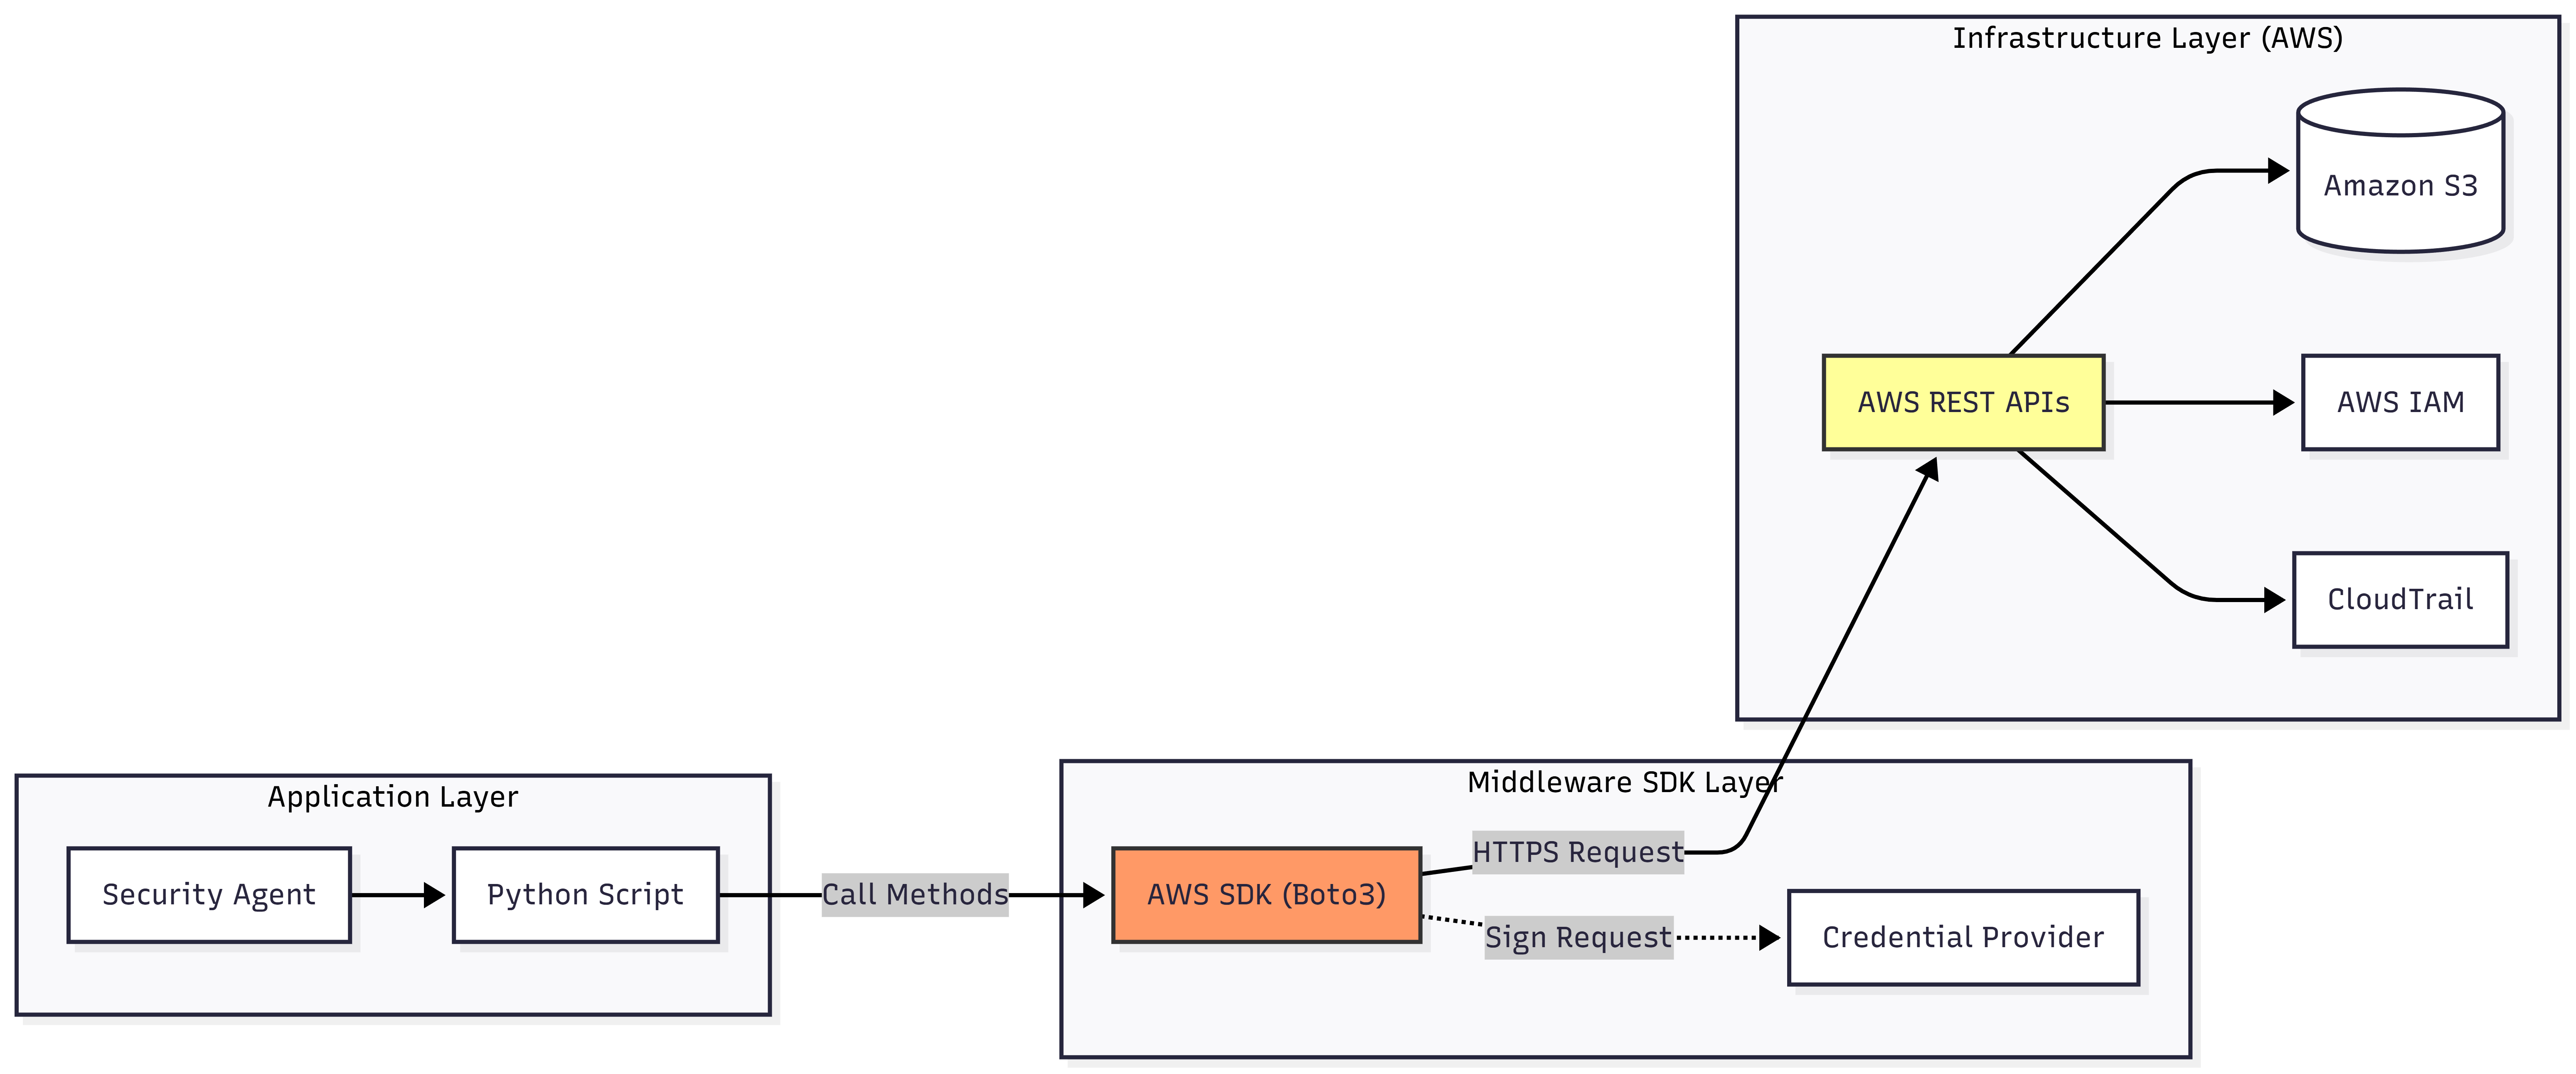
\includegraphics[width=0.8\textwidth]{Images/boto3_architecture.png}
  \vspace{25pt}
  \caption{Cơ chế tương tác giữa ứng dụng Python và AWS thông qua Boto3 SDK (nguồn: tổng hợp từ tài liệu chính thức của AWS \cite{boto3_docs}).}
  \label{fig:boto3_arch}
\end{figure}

\section{Cơ sở dữ liệu vector: ChromaDB}
\label{sec:chromadb_vector}

Cơ sở lý thuyết về vector database, embedding, indexing pipeline, và các chỉ mục ANN (HNSW, IVF) đã được trình bày tại §\ref{subsec:vector-db} và §\ref{subsec:chunking}. Mục này chỉ tập trung vào lý do chọn ChromaDB và cấu hình thực dùng trong đề tài.

\subsection{Vai trò trong hệ thống và cấu hình thực dùng}
\label{subsec:chromadb}

Trong đề tài, \textbf{ChromaDB} \cite{chromadb_docs} đóng vai trò \textit{kho tri thức trung tâm} (Knowledge Hub) cho lớp RAG. Bốn mục tiêu cụ thể: (1) lập chỉ mục các tài liệu Prowler check và AWS Security Maturity Model dưới dạng vector ngữ nghĩa; (2) ánh xạ truy vấn ngôn ngữ tự nhiên của người dùng sang các mã định danh kỹ thuật (Check ID); (3) cung cấp nguồn tham chiếu duy nhất phục vụ grounding cho LLM, giảm hallucination; và (4) duy trì độ trễ truy hồi ở mức mili-giây qua chỉ mục HNSW \cite{malkov2018hnsw}.

Cấu hình thực dùng:
\begin{itemize}
  \item \textbf{Embedding model}: \texttt{BAAI/bge-base-en-v1.5} (768 chiều); được chọn vì điểm MTEB Retrieval cao trên corpus tiếng Anh chuyên ngành bảo mật và chạy được trên CPU với độ trễ chấp nhận được. Truy vấn tiếng Việt được chuẩn hoá sang tiếng Anh qua glossary tất định trước khi embedding (xem §\ref{subsubsec:multilingual_strategy}).
  \item \textbf{Index parameters}: HNSW với \texttt{M=16}, \texttt{ef\_construction=200}, distance metric \texttt{cosine}.
  \item \textbf{Metadata fields}: \texttt{service} (S3, IAM, EC2\dots), \texttt{severity} (Critical/High/Medium/Low), \texttt{control\_id} (CIS, NIST, ISO mapping), \texttt{check\_id} (Prowler), \texttt{source} (AWS docs / CIS Benchmark / AWS SMM).
  \item \textbf{Triển khai}: chế độ \textit{embedded library} trong process Python; persist data ở đường dẫn cục bộ.
\end{itemize}

Cấu hình metadata trên cho phép kết hợp tìm kiếm ngữ nghĩa với bộ lọc cứng: ví dụ truy vấn \textit{``vấn đề S3 nghiêm trọng''} được dịch thành tìm kiếm vector cộng filter \texttt{service = S3 AND severity IN \{Critical, High\}}, giảm nhiễu trong tập kết quả và tăng độ phù hợp với phạm vi kỹ thuật của truy vấn.

\subsection{So sánh với các vector database cùng nhóm}
\label{subsec:vectordb-compare}

Bảng~\ref{tab:vectordb-compare} so các vector database phổ biến theo các tiêu chí quyết định cho đề tài.

\begin{table}[!htb]
\centering
\caption{So sánh các vector database cho RAG cục bộ.}
\label{tab:vectordb-compare}
\footnotesize
\renewcommand{\arraystretch}{1.25}
\setlength{\tabcolsep}{4pt}
\begin{tabular}{|p{2.2cm}|>{\centering\arraybackslash}p{1.6cm}|>{\centering\arraybackslash}p{1.8cm}|>{\centering\arraybackslash}p{1.6cm}|>{\centering\arraybackslash}p{1.6cm}|p{2.6cm}|}
\hline
\textbf{Vector DB} & \textbf{Embedded} & \textbf{Metadata filter} & \textbf{Latency} & \textbf{Production scale} & \textbf{Phù hợp} \\ \hline
\textbf{ChromaDB} \cite{chromadb_docs} & \yesmark & \yesmark Native & ms & Small--medium & \textbf{Chọn}: dev-friendly, đủ cho POC \\ \hline
FAISS \cite{faiss_2017} & \yesmark & \nomark Native & $\mu$s--ms & Medium--large & Tốc độ cao nhưng không có metadata filter native \\ \hline
Qdrant \cite{qdrant_2024} & \nomark Server & \yesmark Native & ms & Large & Production-grade; cần triển khai server riêng \\ \hline
pgvector \cite{pgvector_2024} & \nomark (Postgres) & \yesmark (SQL) & ms & Medium & Tốt nếu đã có PostgreSQL; cần CSDL ngoài \\ \hline
\end{tabular}
\end{table}

ChromaDB được chọn vì cân bằng giữa (i) chế độ embedded không cần server ngoài, phù hợp với phạm vi POC của đề tài, (ii) hỗ trợ metadata filter native, và (iii) tích hợp sẵn với LangChain qua \texttt{Chroma} class. Khi mở rộng quy mô (production-grade), Qdrant hoặc pgvector là lựa chọn nâng cấp tự nhiên.

\section{Tổng kết chương}
\label{sec:literature-synthesis}

Chương này đã hoàn thành ba nhiệm vụ. Thứ nhất, khảo sát bốn nhóm công trình liên quan: CSPM truyền thống và CNAPP thương mại 2024 (§\ref{subsec:rw-cspm}); Compound AI Systems và agentic workflow frameworks (§\ref{subsec:rw-agentic}); LLM ứng dụng cho an ninh mạng (§\ref{subsec:rw-llm-audit}); và đánh giá Security Maturity tự động (§\ref{subsec:rw-maturity}). Đối chiếu trong Bảng~\ref{tab:related-work} cho thấy không công trình nào đồng thời thoả mãn ràng buộc local inference, closed-loop PDCA, HITL native, và maturity-aware --- là gap mà đề tài hướng tới lấp dưới các giả định đã phát biểu tại §\ref{subsec:rw-scope} và bốn câu hỏi nghiên cứu tại §\ref{subsec:rw-rqs}.

Thứ hai, năm công cụ tích hợp đã được giới thiệu cùng lý do chọn cụ thể: Prowler v5 (§\ref{sec:prowler-tool}) làm engine kiểm toán cấu hình với output OCSF; LangChain + LangGraph (§\ref{sec:orchestration-tool}) cho lớp điều phối Compound AI có trạng thái; Ollama + Gemma 3 4B IT (§\ref{sec:slm-tool}) cho local inference; Boto3 (§\ref{sec:boto3_tool}) cho lớp thực thi; ChromaDB (§\ref{sec:chromadb_vector}) cho kho tri thức RAG. Mỗi công cụ được đối chiếu với các candidates trong cùng nhóm qua bảng so sánh để biện minh lựa chọn không chỉ dựa trên \textit{quen thuộc} mà còn dựa trên các tiêu chí kỹ thuật rõ ràng.

Thứ ba, định vị đề tài: kiến trúc đề xuất là một \textbf{Compound AI System} dựa trên LangGraph state-graph, vận hành SLM cục bộ qua Ollama, tích hợp Hybrid RAG (BM25 + Dense + RRF) trên ChromaDB, sử dụng Prowler làm scanner và Boto3 làm actuator, theo chu trình PDCA closed-loop với Human-in-the-Loop tại các điểm phê duyệt nhạy cảm. Hai đóng góp thiết kế đặc trưng --- \textit{Two-Pass Risk Evaluation} (cơ sở lý thuyết tại §\ref{subsec:two-pass-risk}) và \textit{Multi-Query Hybrid RAG} --- sẽ được trình bày chi tiết tại Chương~4. Đánh giá định lượng theo bốn nhóm chỉ tiêu đã giới thiệu tại §\ref{sec:evaluation-methodology} sẽ được trình bày tại Chương~6.

